\documentclass[12pt, a4paper, twoside, openright]{book}

\usepackage{vuwthesis} % sets up some local things, mostly the front page?

\usepackage{palatino} % sets palatino as the default font

\usepackage{url} % for typesetting urls
\usepackage{graphicx}
\usepackage[ruled,vlined]{algorithm2e}
\usepackage[T1]{fontenc}
\usepackage[nottoc,numbib]{tocbibind}
%\renewcommand{\baselinestretch}{1.00}


\begin{document}

\frontmatter
% Book style knows about front matter
% Report style doesn't so you need to set roman numbering etc yourself :-(

%%%%%%%%%%%%%%%%%%%%%%%%%%%%%%%%%%%%%%%%%%%%%%%%%%%%%%%

\title{Using Graph Databases for Automatic Composition of Web Services}
\author{Zhaojiang Zhang}

\subject{Software Engineering}
\abstract{With the rapid development of computer network technology and applications, the demand for services from the internet has grown, as has users? expectation that the internet can provide the services they need. A Web service is a software component that takes input data and produces output data. Since a single Web service provides only limited functionality, in order to complete complex tasks, shared Web services must be used, and it is necessary to combine, or compose these Web services to provide functions needed by users. The objective of service composition is to find a composite service that provides best quality of service (QoS) with the increasing number of available services that can be used for service composition. It is challenging to find a service with optimal QoS efficiently. In this project, we propose an efficient automated QoS-Aware Web service composition approach using graph databases. }
% Books don't normally have abstracts, and this is a bit of a hack

% Uncomment the appropriate degree
\phd
%\mscthesisonly
%\mscwithhonours
%\mscbothparts
% \otherdegree{DEGREE OR DIPLOMA NAME}

\makeatletter
\let\OLDappendix\appendix
\newif\if@appendixinbackmatter
\renewenvironment{appendix}
{
  \if@mainmatter
     \@appendixinbackmatterfalse\OLDappendix
  \else
      \@appendixinbackmattertrue\@mainmattertrue\OLDappendix
\fi
}
\makeatother

%%%%%%%%%%%%%%%%%%%%%%%%%%%%%%%%%%%%%%%%%%%%%%%%%%%%%%%




\maketitle



\tableofcontents


%%%%%%%%%%%%%%%%%%%%%%%%%%%%%%%%%%%%%%%%%%%%%%%%%%%%%%%

% book style knows about mainmatter
% if you are using report style you will have to rest page numbering etc.
\mainmatter

%%%%%%%%%%%%%%%%%%%%%%%%%%%%%%%%%%%%%%%%%%%%%%%%%%%%%%%

% individual chapters included here

\chapter{Introduction}\label{C:intro}
Service-Oriented Architecture (SOA) \cite{1} is an architectural style for building software applications which uses services available in a network. SOA is realised through a standards-based technology called Web services, which allows coupling between Web services, so they can be reused. A Web service is a self-contained unit with limited functionality, that takes input data and produces output data. To provide value-added functions, it is necessary to compose Web services to provide powerful service functions. The result of such composition is to take a set of input data provided by the user and create a corresponding set of output data needed by a user.  

Currently there are three main approaches to Web service Composition. The first group of approaches includes several those which employ traditional methods such as Integer Linear Programming (ILP) \cite{7} to solve the problem of Web service composition. These approaches lack scalability and are no longer efficient since the number of Web services is increasing extraordinarily quickly. The second group includes various Evolutionary Computing (EC) approaches, such as Genetic Algorithms (GA) \cite{8}, Genetic Programming(GP) \cite{14,2,9} and Particle Swarm Optimisation (PSO) \cite{10,19}. These approaches are slow, especially when checking the dependencies between the component services, a task which requires a substantial amount of resources. The third type is the graph based approach, such as \cite{13,5}. This approach stores graph dependencies in memory temporarily rather than saving them permanently on local storage.


\section{Aims and Objectives}
The aim of this project is to propose an efficient automated QoS-aware Web service composition approach using Graph Databases. Existing Web service composition approaches \cite{2, 4} do not permanently store Web service dependencies, which means that when running the composition algorithm for different tasks, the algorithm will keep Web service dependencies in memory. The problem with this is that when a new task needs to be carried out, it becomes necessary to regenerate its Web service dependencies. This is because different tasks have different enquire (input) and result (outputs) data, upon which Web service dependencies are based. In practice, this behaviour dramatically increases the cost of running the system, since Web service dependencies which need only be generated once may in fact be generated several times. Moreover, the existing approach requires the generation of a corresponding workflow after each composition has been established. This takes a substantial amount of time and slows down the entire process.


Graph databases store data and relationships between data as graphs. In this project we employ a graph database to store the dependencies between services in a service repository and our service composition approach is based on the use of these graph databases. This project aims to create a graph database-based approach that generates Web service solutions efficiently by reducing the composition costs involved in checking dependencies of services. 

To achieve the aim of the project, the project is conducted with the following objectives:
\begin{enumerate}
  \item To review existing works in literature on this topic.
  \item To use a graph database to model and store services and their dependencies within a service repository.
  \item To generate non-QoS-aware Web services compositions with no redundant services in the compositions.
  \item To select service compositions with the best QoS. 
  \item To conduct a full evaluation of our approach by comparing the performance of our proposed approach with one of the existing approaches.
\end{enumerate}



\section{Structure of Report} 
This remainder of the report is organised as follows: A background and literature review is presented in Chapter 2. Chapter 3 gives a description of our Graph database-based approach. Chapter 4 covers our evaluation to compare the performance of our approach with an existing approach.  The final section of this report presents our conclusions regarding our approach, and proposes possible future developments regarding our approach.



\chapter{Background and Literature Review}\label{C:ex}
\section{Background}
\subsection{QoS Properties}
Quality of service (QoS) is one of the important factors to consider when composing services. It defines the non-functional requirements of a service, such as response time, execution cost, availability, reliability etc. Good quality of service means achieving certain QoS goals which are termed QoS values or QoS properties. These QoS properties indicate whether a Web service is reliable, trustworthy or efficiency. Their significance stems from the fact that a Web service may be functionally capable of performing a given task, but might not be reliable or efficient enough to achieve users' satisfaction. Web services are usually rated using multiple QoS values, each value representing an aspect, or QoS property, of the Web service. QoS properties are the most commonly used characteristics for measuring the quality of Web services and even composite services, as they indicate whether a service is capable of meeting users' expectations.\par

To model the performance of service compositions we considered four QoS attributes: availability, reliability, execution cost and response time. We chose these because they are commonly used in this field \cite{4,14,15,16}. \par
According to \cite{4,11,18}, the four above-mentioned QoS properties are defined as follows:\par

Execution Cost is the amount of money that a service requester has to pay for using the Web service. The global execution cost of a composite set of services can be treated as the sum of the execution costs of all the operations invoked by the services used. For example, the total execution cost of the composite service in Figure \ref{fig:process} is total execution $C = C(S_{1}) + Cost(S2) + Cost(S3) + Cost(S4)$.$w_{1} + w_{2} + w_{3} + w_{3} = 1$.\par
The response time of a single task is the time which elapses between sending a task request and receiving a response. Web service composition allows services to execute in parallel. Thus, when considering a step where two tasks execute in parallel, the path with the longest response time is chosen to calculate the time taken for that step.\par
For example, in Figure \ref{fig:process}, which shows an example Web service composition, services \emph{S2} and \emph{S3} can be executed in parallel. The response time depends on S2 and S3's local QoS duration property values. If S2's QoS duration property value is greater than S3's QoS duration property value, then the overall response time of the composite service can be computed as the sum of all three service nodes S1, S2 and S4's local QoS duration property values.\par
Availability is defined as the ratio of (1) the time during which a service is ready for use and (2) the time during which the Web service exists. The global availability of a composite Web services can be computed as the product of the local availabilities of the Web services used in the service composition.  For example, the availability of the composite service in Figure 2.1, can be computed as Availability(S1) x Availability(S3) x  Availability(S2) x Availability(S4). \par
Reliability is the how reliable message delivery is to the Web service within the maximum permitted time frame. Global reliability can be calculated as the product of the local reliabilities of the Web services used in the service composition. For example, the reliability of the composite service in Figure 2.1, can be computed as Reliability(S1) x Reliability(S3) x Reliability(S2) x Reliability(S4). \par
\begin{figure}[H]
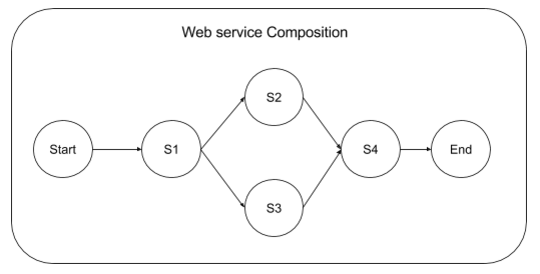
\includegraphics[width=9cm]{Figure2-1ExampleWebServiceComposition.png}
\centering
\caption{Example Web service composition}
\end{figure} 
\subsection{Neo4j graph database}
We employed a Neo4j \cite{6} graph database for our project because it is suitable for representing connected and directed Web services and it allows for very fast retrieval, traversal and navigation of data. A Neo4j Graph Database stores all its data in Nodes and Relationships. All Nodes and Relationships have their own individual properties. And for each data set we need only create a graph database once, after which we can use this database to solve different composition problems. \par

\section{Literature Review}
Over the past few years, Web services have become widely used. A large number of complex applications can be developed using compositions of existing services. Automatic Web service composition technology has become a major focus and challenge in building robust applications which make use of distributed services which provide various functions. Many approaches have been developed for Web service composition, but only a few of them use the concept of graph theory. In this section, we will present a brief overview of some graph-based techniques that deal with automatic Web service composition.\par
Da Silva A. S.et al. presents in \cite{2} an evolutionary computation technique that performs fully automated Web service composition using graph representations for solutions. There are two steps. The first step is to initialise the population by employing a graph building algorithm based on the planning graph approach described in composition literature \cite{3}. The second step is to perform mutation and crossover operations on selected candidates, to generate a new set of candidates and evaluate the fitness of those candidates.\par
The drawback of the approach in \cite{2} is that the graph mutation space contains a lot of invalid service compositions that either violate the constraints of service dependencies or deteriorate the overall performance. Another disadvantage is that the system saves all the Web service dependencies in memory. With every new service request, this approach needs to regenerate all the dependencies again which incurs expensive computation costs. Furthermore, the cost of executing the graph building algorithm is high, since the graph building algorithm is employed twice, in two different processes, namely in the process of generating initial populations and the process of performing mutation and crossover operations.\par
Seyyed, V., H et al. \cite{5} uses a graph search algorithm to construct Web service compositions. This algorithm is based on input-output dependencies of Web services. In order to solve the service composition problem, the authors divide the process into two steps. The first step is to look for Web services which can potentially participate in the composition, and the second step is to find a corresponding composition. The graph building algorithm constructs edges between directly related Web services which have data dependencies between the inputs and outputs of these services. The main shortcoming of this approach is that semantic functions are not considered in the dependencies between input and output parameters. Thus there is no guarantee that a generated composite service will provide the precise functionality requested by the user.\par
The Web service composition approaches proposed by Da Silva A. S.et al. et al. in \cite{2} and Seyyed, V., H et al. in \cite{5}, also share a common drawback. They don't include quality of service in their approach. This means the resulting Web services may not perform tasks that meet a user's non-functional requirements.\par
As we seen above, existing graph-based approaches need to build a data dependency graph for each given task. However, database dependencies between services in a service repository remain stable for all service tasks. Therefore, once a service dependency graph is generated it is best stored and used for all service tasks. In this project we propose to use a graph database to store the information related to services and dependencies of services of a service repository. With each new service task we can utilize existing dependency information contained within graph database dependency graphs. Our approach also takes quality of service (QoS) into consideration by including QoS properties with each edge between Web services.    
\include{workdone}
\chapter{Future Plan and Conclusions}\label{C:con}

This report introduces the use of Neo4j graph databases to model QoS-aware web service compositions. The proposed five algorithms can efficiently create the database, reduce the database, and generate an initial population. The proposed algorithm can automatically construct a relatively good initial population. Our evaluation results have verified the correctness of web service compositions created using our algorithms.

Currently, our proposed method is only able to generate initial populations. In the second part of the project, we will use QoS to calculate global optimisation to find better web service compositions. We may consider using GP to improve initial populations by using mutation and crossover operators.

The first task for future work is to design a fitness function to produce solutions with the smallest possible number of service nodes and with the shortest possible paths from the start node to the end node. The second task for future work is to build QoS-aware compositions and calculate the global optimisation and improve the results. The third task for future work is to analyse and design the evaluation by comparing the performance of our system against the traditional GP approach and other GP approaches.  The Figure 4.1 shows the current working progress. As shown in Figure 4.1, our objectives 1, 2, and 3 have been achieved. The rest of our work is to analyse more preliminary evaluations and start on design work for objectives 4 and 5 early enough to be able to revisit and modify objective 3 if needed.\\

\begin{figure}[h]
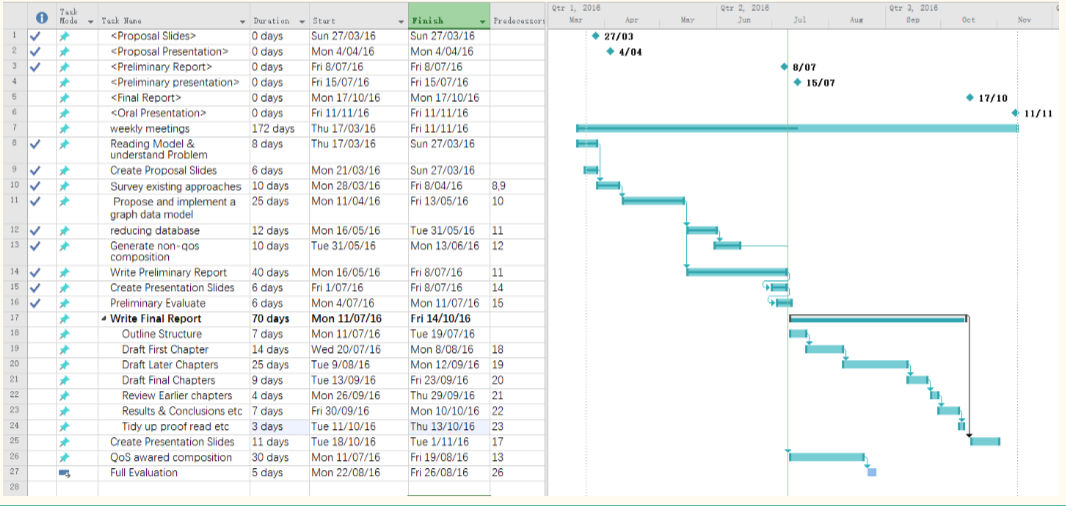
\includegraphics[width=15cm]{ganttChart.png}
\centering
\caption{GANNT CHART}
\end{figure}



%%%%%%%%%%%%%%%%%%%%%%%%%%%%%%%%%%%%%%%%%%%%%%%%%%%%%%%
% and of course book style knows about backmatter
% \backmatter caused problems with appendices :-(
% and of course report style doesn't
%%%%%%%%%%%%%%%%%%%%%%%%%%%%%%%%%%%%%%%%%%%%%%%%%%%%%%%

\renewcommand\bibname{References} 
%\bibliographystyle{ieeetr}
\bibliographystyle{acm}
\bibliography{ref}
\appendix
\chapter{Appendix: Project Proposal Slides}
\begin{figure}[h]
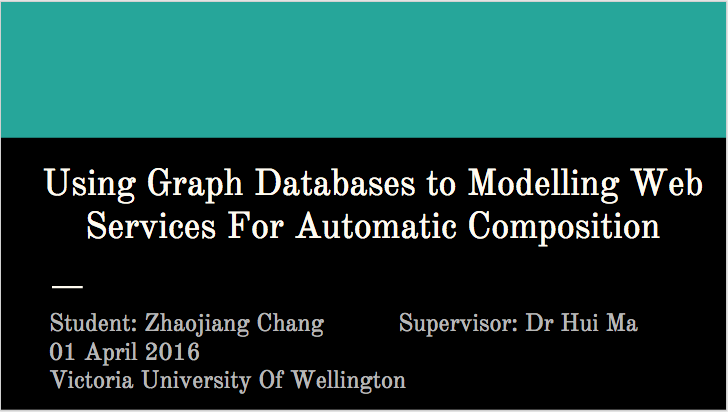
\includegraphics[width=15cm]{1.png}
\centering
\caption{slide 1}
\end{figure}

\begin{figure}[h]
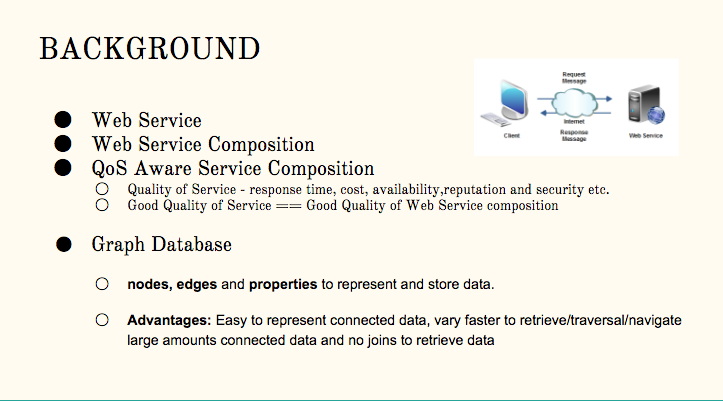
\includegraphics[width=15cm]{2.png}
\centering
\caption{slide 2}
\end{figure}

\begin{figure}[h]
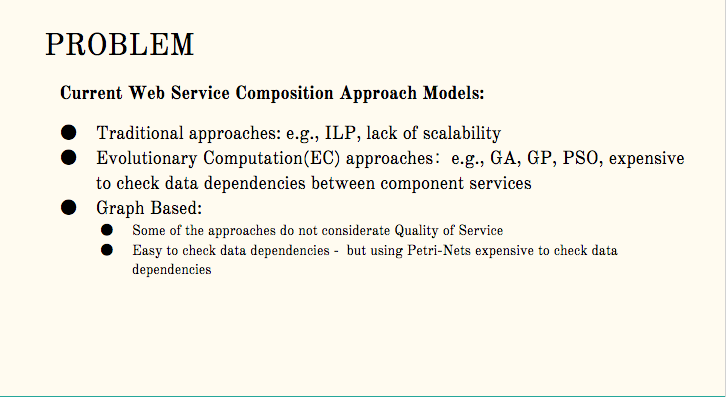
\includegraphics[width=15cm]{3.png}
\centering
\caption{slide 3}
\end{figure}

\begin{figure}[h]
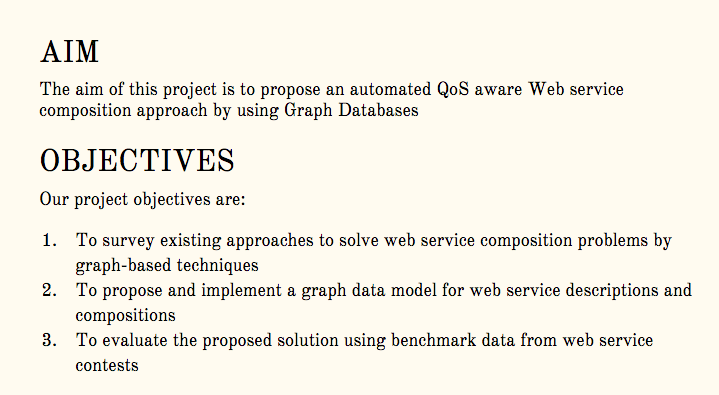
\includegraphics[width=15cm]{4.png}
\centering
\caption{slide 4}
\end{figure}

\begin{figure}[h]
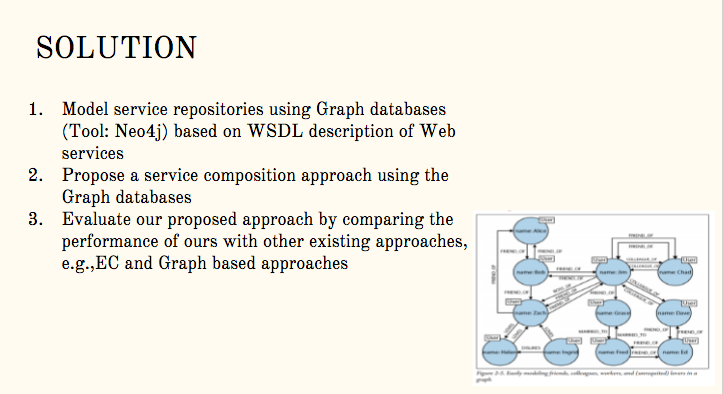
\includegraphics[width=15cm]{5.png}
\centering
\caption{slide 5}
\end{figure}

\begin{figure}[h]
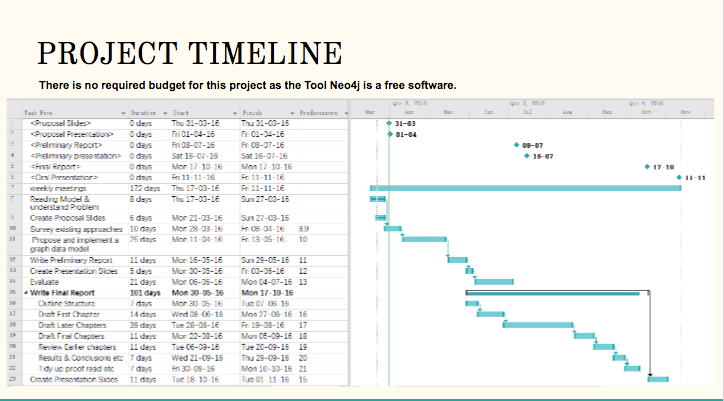
\includegraphics[width=15cm]{6.png}
\centering
\caption{slide 6}
\end{figure}



\end{document}
